\subsection{Spectra}\label{sec:spectra}
%schriste - this section needs major work

%ayshih - this whole paragraph can be deleted
Spectroscopy consists in the study of the radiative energy related to the wavelength.
An spectrum is normally obtained by observing a range of frequencies at the same time; 
it can be measured for example in radio wavelengths by a frequency sweep with 
a radio receiver or in visible and ultraviolet by the dispersion of the incident light 
through a diffraction grating or prism.
The analysis of the resultant spectrum can provide properties of the plasma observed 
such temperature, density, speed, etc.
Therefore, spectroscopy provides to the solar physicists invaluable information about 
the composition and the physical properties of the Sun.  

SunPy aims to provide broad support for solar spectroscopy instruments, however the 
variety and complexity of such datasets makes it very challenging to add support to them all 
in a general way.
The \texttt{spectra} module implements a \texttt{Spectrum} class for 1D data
(intensity versus frequency) and a \texttt{Spectrogram} class for 2D data
(intensity versus time and frequency.
Each of these classes use a \texttt{numpy.ndarray} class as its \texttt{.data} attribute.
These two classes were implemented by funding provided by the Astrophysics Research 
Group at Trinity College Dublin.

As of SunPy 0.4, the \texttt{Spectrogram} class supports radio spectra from the e-Callisto 
solar radio spectrometer network (\url{http://www.e-callisto.org/})
and STEREO/SWAVES spectrograms.
As with other SunPy data types, the \texttt{Spectrogram} class has been
built so each instrument initialises using a subclass containing the instrument-specific 
functionalities.
The common functionality provided by the base \texttt{Spectrogram} class includes
reading data,
joining different time ranges and frequencies,
performing frequency-dependent background subtraction,
and convenient visualization and sampling of the data.

Listing \ref{code:spectra} shows how the \texttt{CallistoSpectrogram} object retrieves
from the online data archive the files that are between the time range specified and
the observatory of interest.  In this case the data is requested from \textit{BIR},
which is the code name of the
Rosse Observatory at Birr Castle in Ireland (\url{http://www.rosseobservatory.ie}).
When the data is requested using the \texttt{.from\_range} function, the object merges
into a single spectrogram all the files downloaded, each with 15 minutes observation data 
and in some cases with different files for different frequency ranges.  
In the example shown here BIR observed in two frequency ranges: 20--90\,MHz and 55--355\,MHz.
Since the data is not evenly spaced in the frequency range, the \texttt{Spectrogram} object
linearise the frequency axis for a better analisys, as shown in the resultant figures.
It is also shown in the example the effect of the implemented background substraction and
\texttt{.peek} method.

\begin{listing}[H]
\begin{minted}[bgcolor=bg]{pycon}
>>> from SunPy.spectra.sources.callisto import CallistoSpectrogram
>>> tstart, tend = "2011-06-07T06:00:00", "2011-06-07T07:45:00"
>>> callisto = CallistoSpectrogram.from_range("BIR", tstart, tend)
>>> callisto_nobg = callisto.substract_bg()
>>> callisto_nobg.peek(vmin = 0)
\end{minted}
\begin{center}
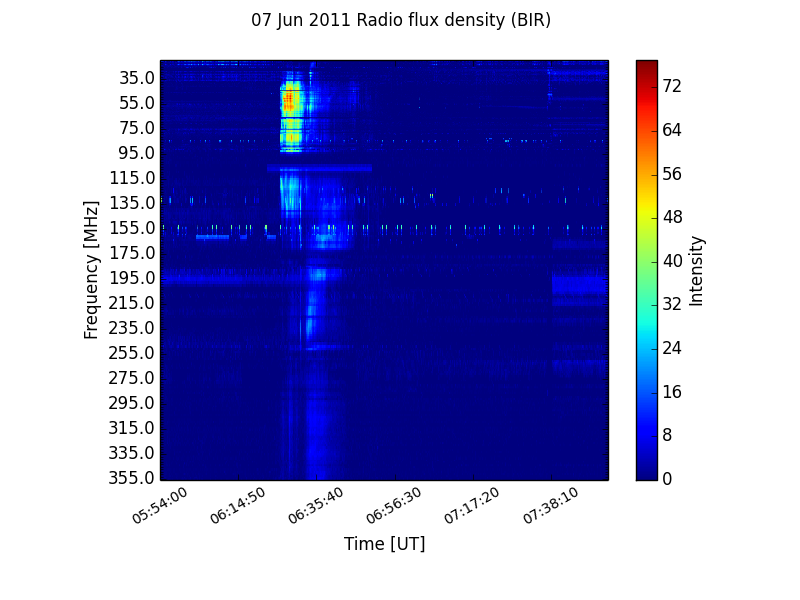
\includegraphics[width=0.8\columnwidth]{callisto_nobg}
\end{center}
\caption{Example of how \texttt{CallistoSpectrogram} retrieves the data
for the time range and observatory requested, merges it all and removes the background
signal.}
\label{code:spectra}
\end{listing}

% Download Callisto
% Merge multiple time-ranges / frequencies (just work from downlad!)
% Merge callisto with swaves

